\documentclass{slides}

\lstset{language=C++}

\usepackage{xspace}
\newcommand{\ie}{\textit{i.\thinspace e.}\xspace}
\newcommand{\eg}{\textit{e.\thinspace g.}\xspace}
\usepackage{tikz}
\usetikzlibrary{shapes,positioning}

\begin{document}

\graphicspath{{figures/}}

\title[The Compilation Process]{\Large The Compilation Process}

\author[O. Lenz]{Olaf Lenz} 
\institute{Institut für Computerphysik\\Universit\"at Stuttgart}
\date{March 17-21, 2014}

\setbeamertemplate{footline}{}
\begin{frame}
  \titlepage
\end {frame}
\setbeamertemplate{footline}[icp]

\begin{frame}
  \frametitle{Separate Compilation}
  \begin{columns}[T,onlytextwidth]
    \column{0.5\textwidth}
    \begin{itemize}
    \item So far, all programs were a single file
    \item Large software projects consist of thousands of lines of
      code
    \item Problem:
      \begin{itemize}
      \item Bad for team projects
      \item Compilation may take very long
      \item Impractical to edit
      \end{itemize}
    \item Better: split the project into several files, \emph{compile}
      them one by one and \emph{link} them together at the end
    \end{itemize}

    \column{0.5\textwidth}
    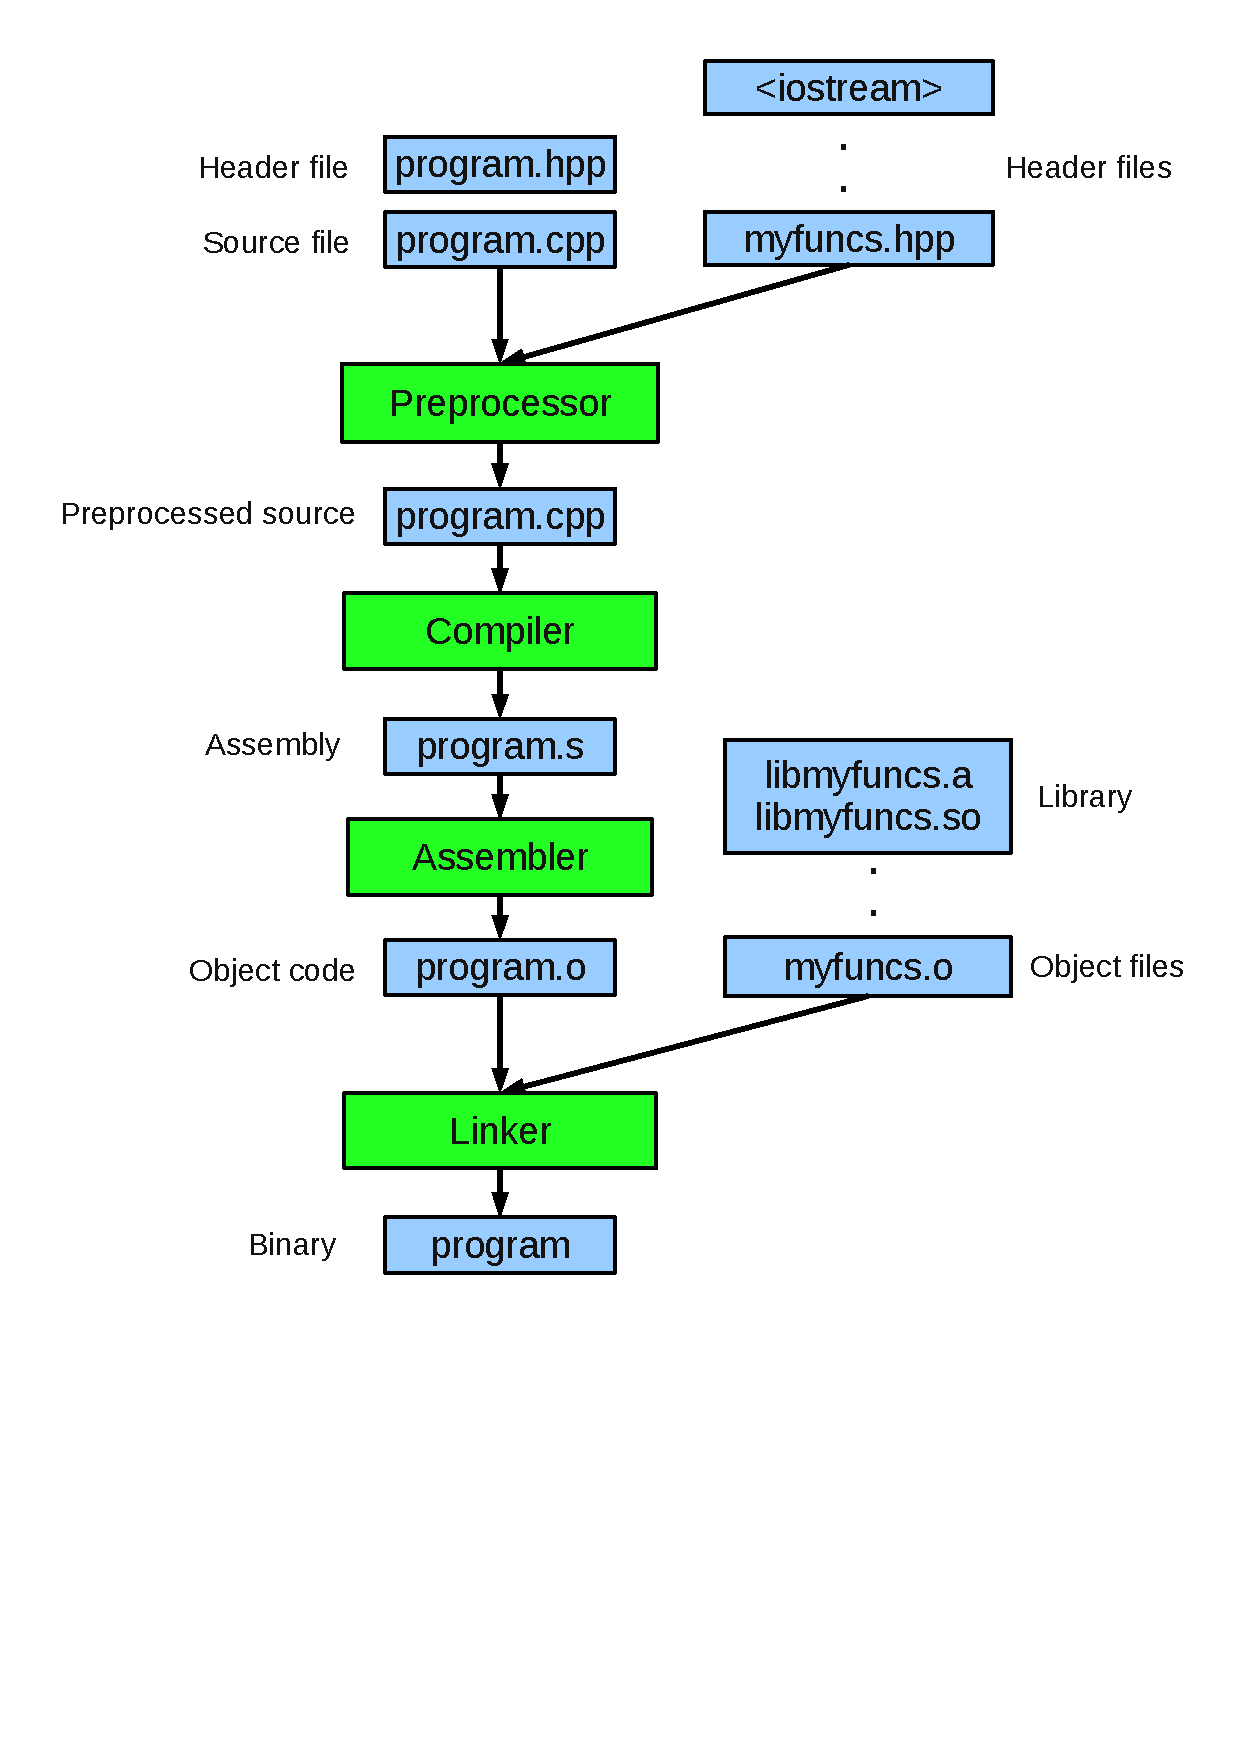
\includegraphics[height=1.1\textheight]{compilation}
  \end{columns}
\end{frame}

\begin{frame}[fragile]
  \frametitle{Stage 1: Preprocessor Inclusions}
  \begin{columns}[T,onlytextwidth]
    \column{0.5\textwidth}
\begin{lstlisting}[language=bash]
g++ -E <source>
\end{lstlisting}
\begin{lstlisting}
#include FILE
\end{lstlisting}
    \begin{itemize}
    \item Preprocess FILE, output \lstinline!.cpp!-file
    \item Pure text replacement: \lstinline!#include FILE! is replaced
      by the contents of FILE
    \item Outputs a single C++ file
    \end{itemize}

    \column{0.5\textwidth}
    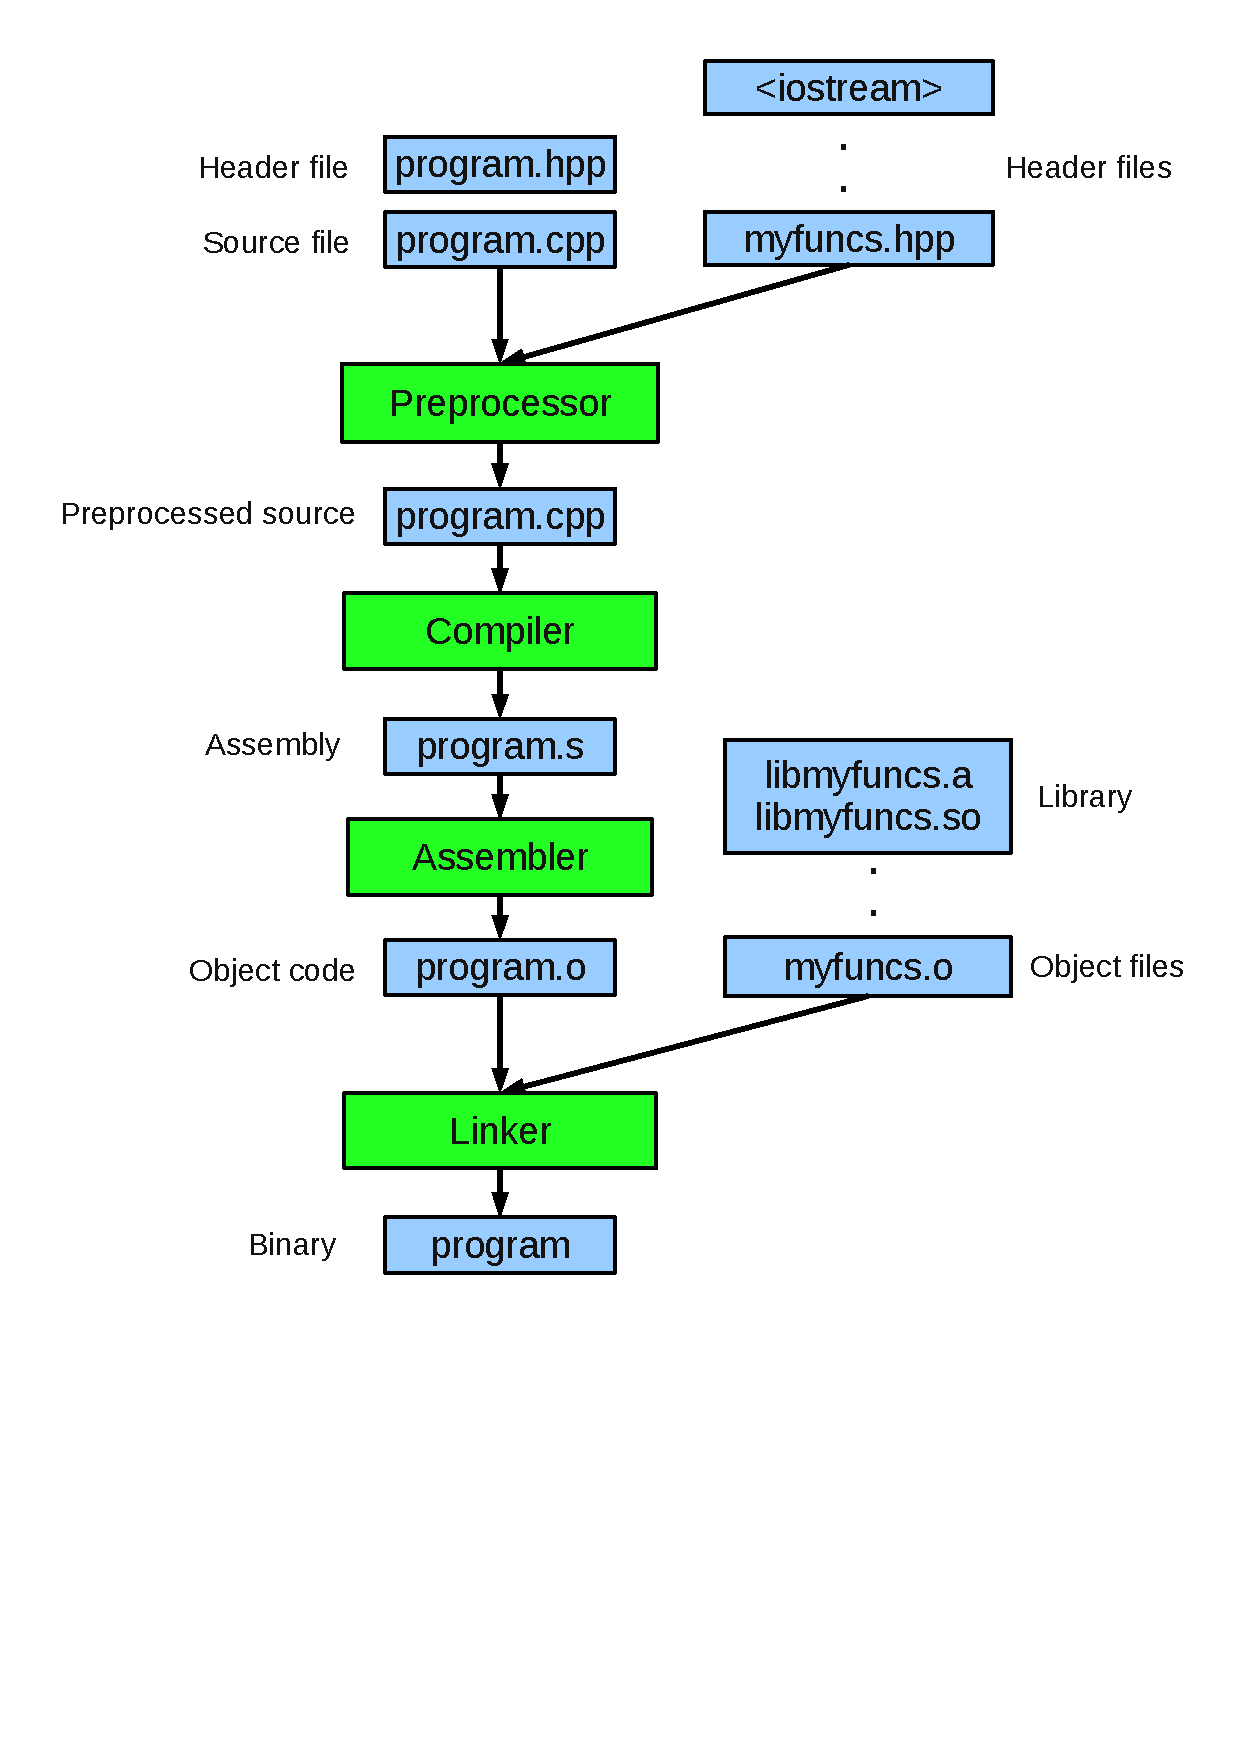
\includegraphics[height=1.1\textheight]{compilation}
  \end{columns}
\end{frame}

\begin{frame}[fragile]
  \frametitle{Stage 1: Preprocessor Macros}
  \begin{itemize}
  \item \lstinline!#define NAME REPLACEMENT! defines a
    \emph{macro} with the given NAME
  \item Whenever the macro name turns up in the file, it is replaced
    by the REPLACEMENT
  \item This \emph{was} used for constants (\eg \lstinline!M_PI!)
  \item Preprocessor Conditionals
    \begin{lstlisting}
#ifdef MACRO
.
.
#else
.
.
#endif
    \end{lstlisting}
  \item Nowadays mostly used for compile time guards
  \end{itemize}
\end{frame}

\begin{frame}[fragile]
  \frametitle{Declarations vs. Definitions}
  \begin{columns}[T,onlytextwidth]
    \column{0.5\textwidth}
    \begin{itemize}
    \item Not all code is open source, so not all code should be there.
    \item $\Rightarrow$ build object code from your code, and link it
      together.
    \item Problem: To be able to compile a function, some things must be
      known about all functions, variables and types that occur.
\begin{lstlisting}
int main() {
  cout << "Hello, World!" << endl;
}    
\end{lstlisting}
    \item What is \lstinline!cout!, \lstinline!<<! and \lstinline!endl!?
    \item $\Rightarrow$ Split function into declaration and definition
    \end{itemize}

    \column{0.5\textwidth}
    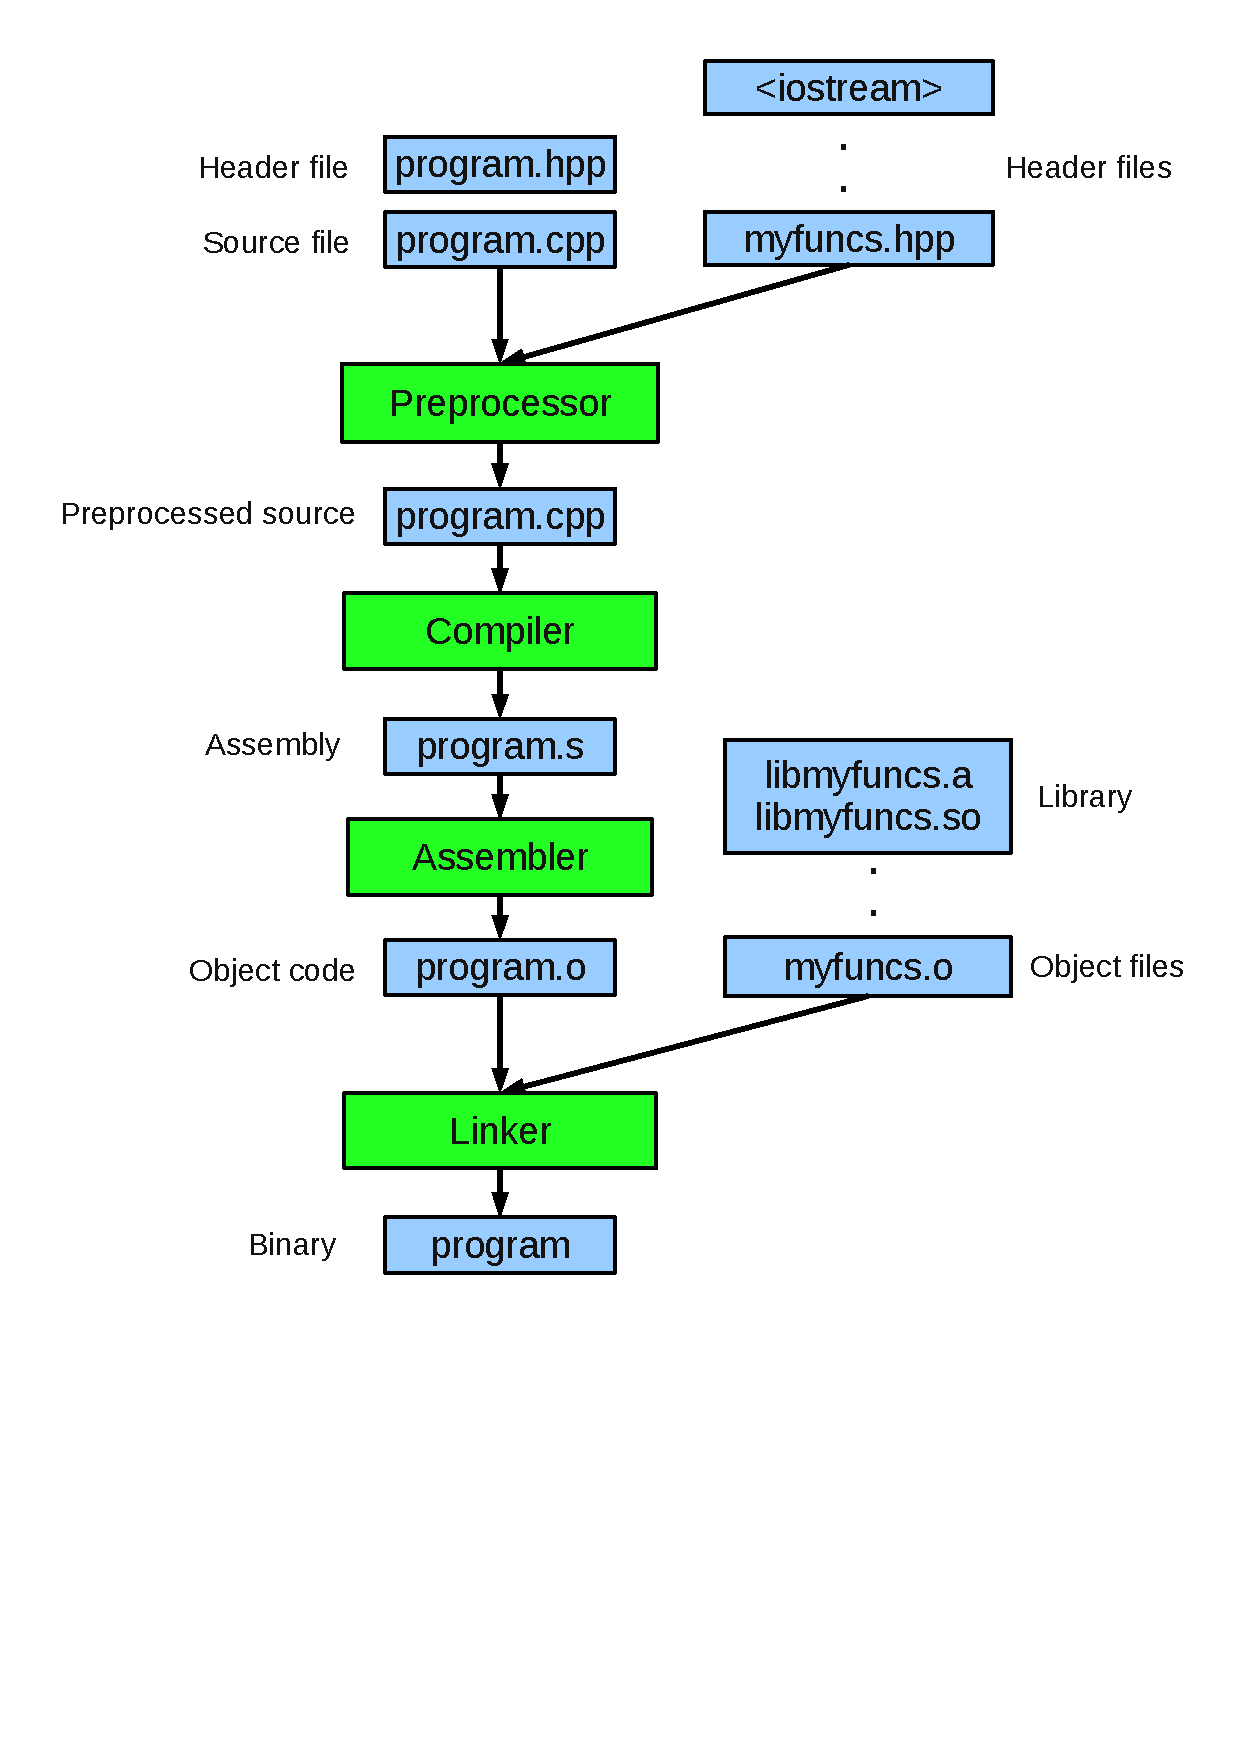
\includegraphics[height=1.1\textheight]{compilation}
  \end{columns}
\end{frame}

\begin{frame}[fragile]
  \frametitle{Declarations vs. Definitions}
  \begin{itemize}
  \item All functions and variables (\emph{symbols}) in C++ can be
    \emph{declared} and have to be \emph{defined} somewhere
  \item The \emph{declaration} of a symbol introduce names to the
    compiler: ``This function or this variable exists somewhere and
    here is what it should look like.''
  \item The \emph{definition} tells the compiler: ``Make this variable
    or function here.''
  \item Declarations can be repeated, definitions must be unique
  \item A \emph{header file} (\eg \texttt{.hpp}) should only contain
    declarations (it is included in other header and source files)
  \item A \emph{source file} (\eg \texttt{.cpp}) contains definitions
    as well as declarations
  \item All symbols declared in a header file should be defined in
    exactly one source file
  \end{itemize}
\end{frame}

\begin{frame}[fragile]
  \frametitle{Function Declarations and Definitions}
  \begin{itemize}
  \item Declaration
    \begin{lstlisting}
int func(int length, int width);
    \end{lstlisting}
  \item Provides the signature (name, parameters and return type) of a
    function
  \item The names are ignored by the compiler
  \item Definition
    \begin{lstlisting}
int func(int length, int width) {
  // function code
  .
  .
}
    \end{lstlisting}
  \end{itemize}
\end{frame}

\begin{frame}[fragile]
  \frametitle{Variable Declarations and Definitions}
  \begin{itemize}
  \item Only interesting for \emph{global variables}
  \item Declaration
    \begin{lstlisting}
extern int a;
    \end{lstlisting}
  \item Definition
    \begin{lstlisting}
int a;
    \end{lstlisting}
  \end{itemize}
\end{frame}

\begin{frame}[fragile]
  \frametitle{Stage 1: Preprocessor Inclusions 2}
  \begin{columns}[T,onlytextwidth]
    \column{0.5\textwidth}
    \begin{lstlisting}[language=bash]
g++ -E -I<path> <source>
    \end{lstlisting}
    
    \begin{itemize}
    \item The header files have to be in the \emph{include path}
      \begin{itemize}
      \item Usually called \texttt{.../include} on a Unix system.
      \item The default include path contains \eg \texttt{/usr/include}.
      \item It can be extended in the compiler call by \texttt{-I
          <path>}.
      \item \lstinline!#include <file>! for system headers
      \item \lstinline!#include "file.hpp"! for own headers
      \end{itemize}
    \end{itemize}

    \column{0.5\textwidth}
    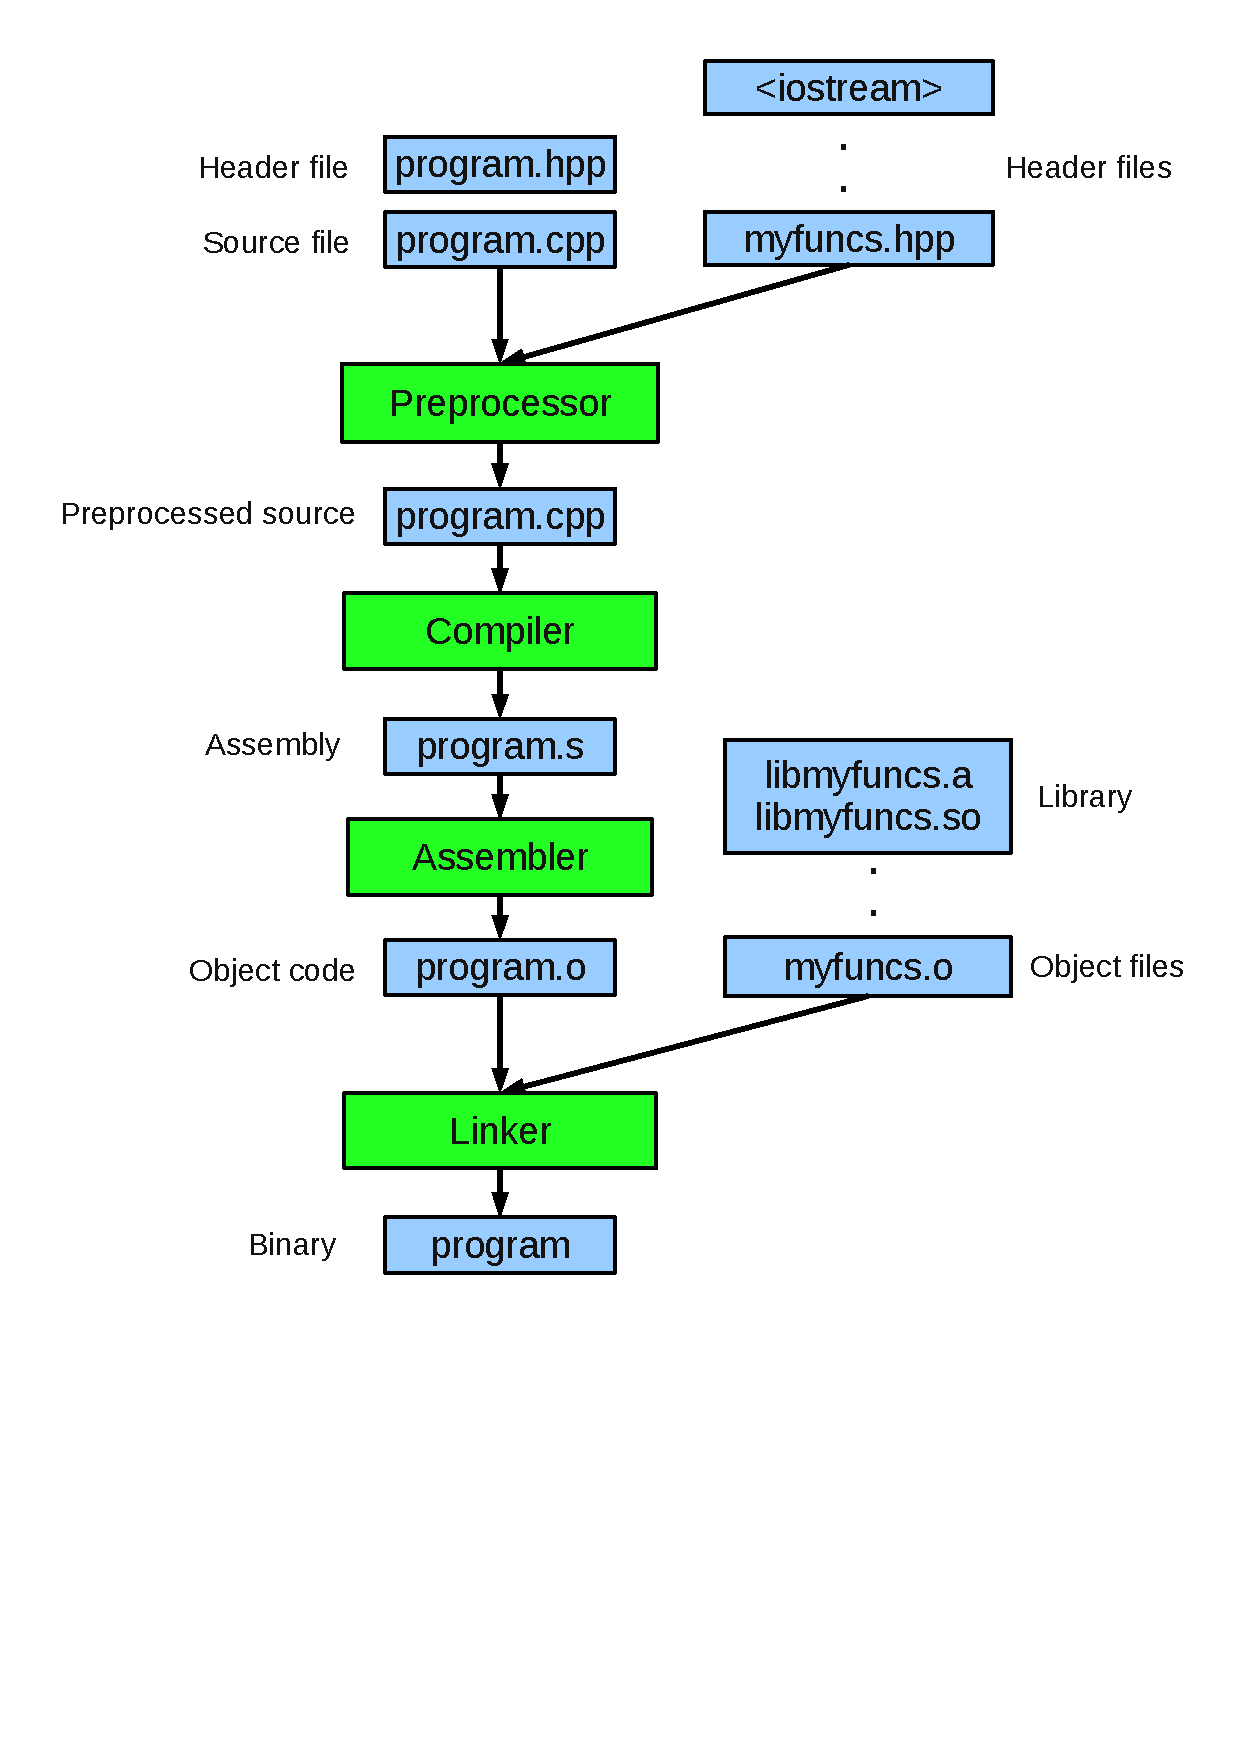
\includegraphics[height=1.1\textheight]{compilation}
  \end{columns}
\end{frame}

\begin{frame}[fragile]
  \frametitle{Preprocessor Compile Time Guards}
    \begin{itemize}
    \item If a header is included several times, this prevents
      multiply definitions of types
      \begin{lstlisting}
#ifndef __MYHEADER_HPP
#define __MYHEADER_HPP
.
// The actual code
.
#endif          
      \end{lstlisting}
    \item Or they can be used for conditional compilation, \eg when a
      program can use a library if it is there, but can still work
      if not
      \begin{lstlisting}
#ifdef FFTW
// code that uses FFTW
#else
// code without FFTW
#endif        
      \end{lstlisting}
    \end{itemize}
\end{frame}

\begin{frame}[fragile]
  \frametitle{Stage 2: Compiler}

  \begin{itemize}
  \item Performs \emph{static type checking}: do the types match?
  \item The \emph{code generator} translates source code into machine
    code, function by function
  \item An \emph{optimizer} optimizes the machine code
  \item Complains when a symbol is used that has not been declared
  \item \dots but does \emph{not} complain when it is not defined!
  \item For each \emph{defined symbol} in the code, it will store the
    generated machine code together with the symbol
  \item For each \emph{undefined symbol} that is used in the code and
    that was only declared but not defined, it will store where it is
    used
  \end{itemize}
\end{frame}

\begin{frame}[fragile]
  \frametitle{Stage 2: Compiler 2}
  \begin{columns}[T,onlytextwidth]
    \column{0.5\textwidth}
  \begin{itemize}
  \item It generates \lstinline!.o!-files (\emph{object
      code}-files) (nothing to do with OOP objects!)
  \item \lstinline!g++ -c FILE!: Preprocess and compile FILE, output
    \lstinline!.o!-file
  \item \lstinline!nm -C FILE.o!: Shows defined and undefined symbols
    in \lstinline!.o!-file
  \end{itemize}
    \column{0.5\textwidth}
    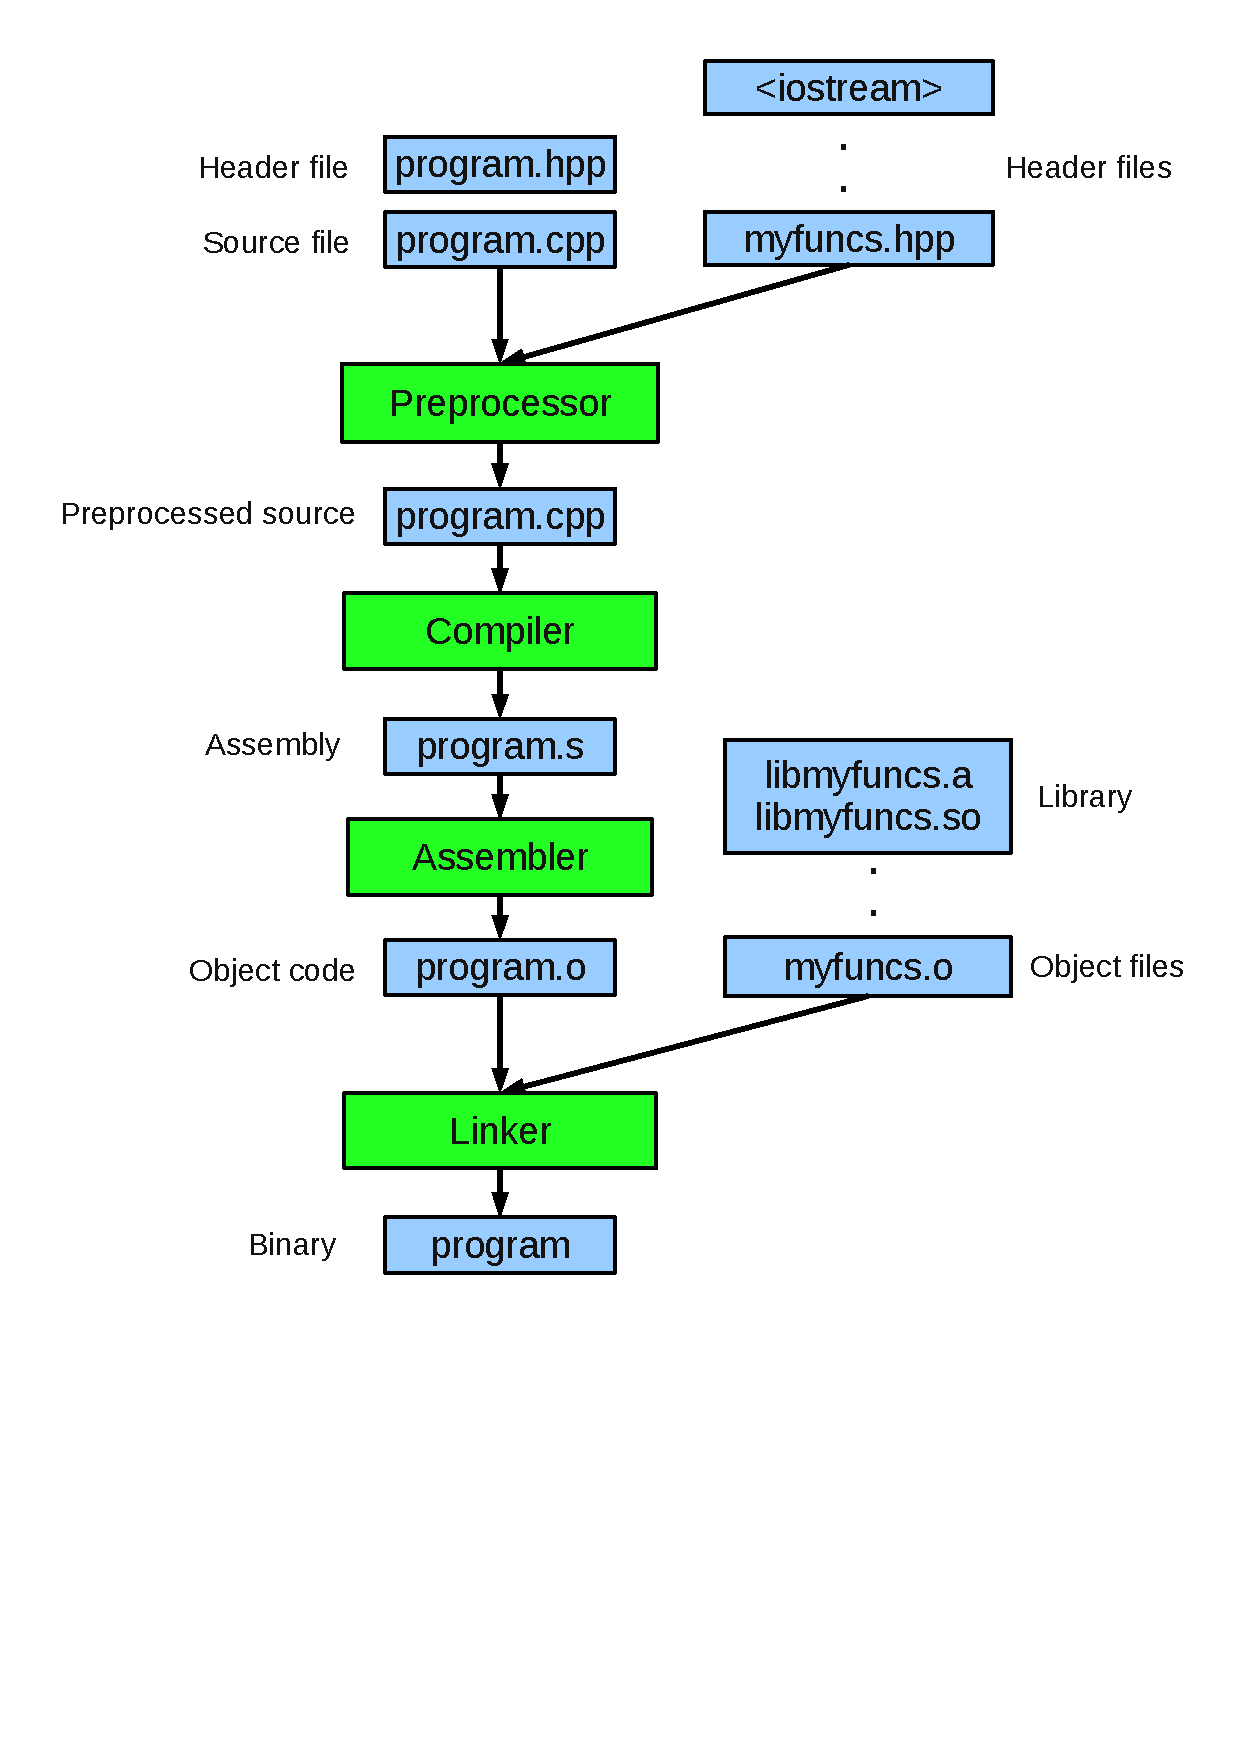
\includegraphics[height=1.1\textheight]{compilation}
  \end{columns}
\end{frame}

\begin{frame}[fragile]
  \frametitle{Stage 3: Linker}
  \begin{columns}[T,onlytextwidth]
    \column{0.5\textwidth}
  \begin{itemize}
  \item \emph{Links} several \lstinline!.o!-files together into a
    single executable file
  \item Starts with the function \texttt{main}
  \item Recursively \emph{resolves} all undefined symbols
    \begin{itemize}
    \item puts the code of used symbols into the executable
    \item puts the addresses of the symbol where the symbol is used
    \end{itemize}
  \item Fails when a symbol cannot be resolved
  \end{itemize}
    \column{0.5\textwidth}
    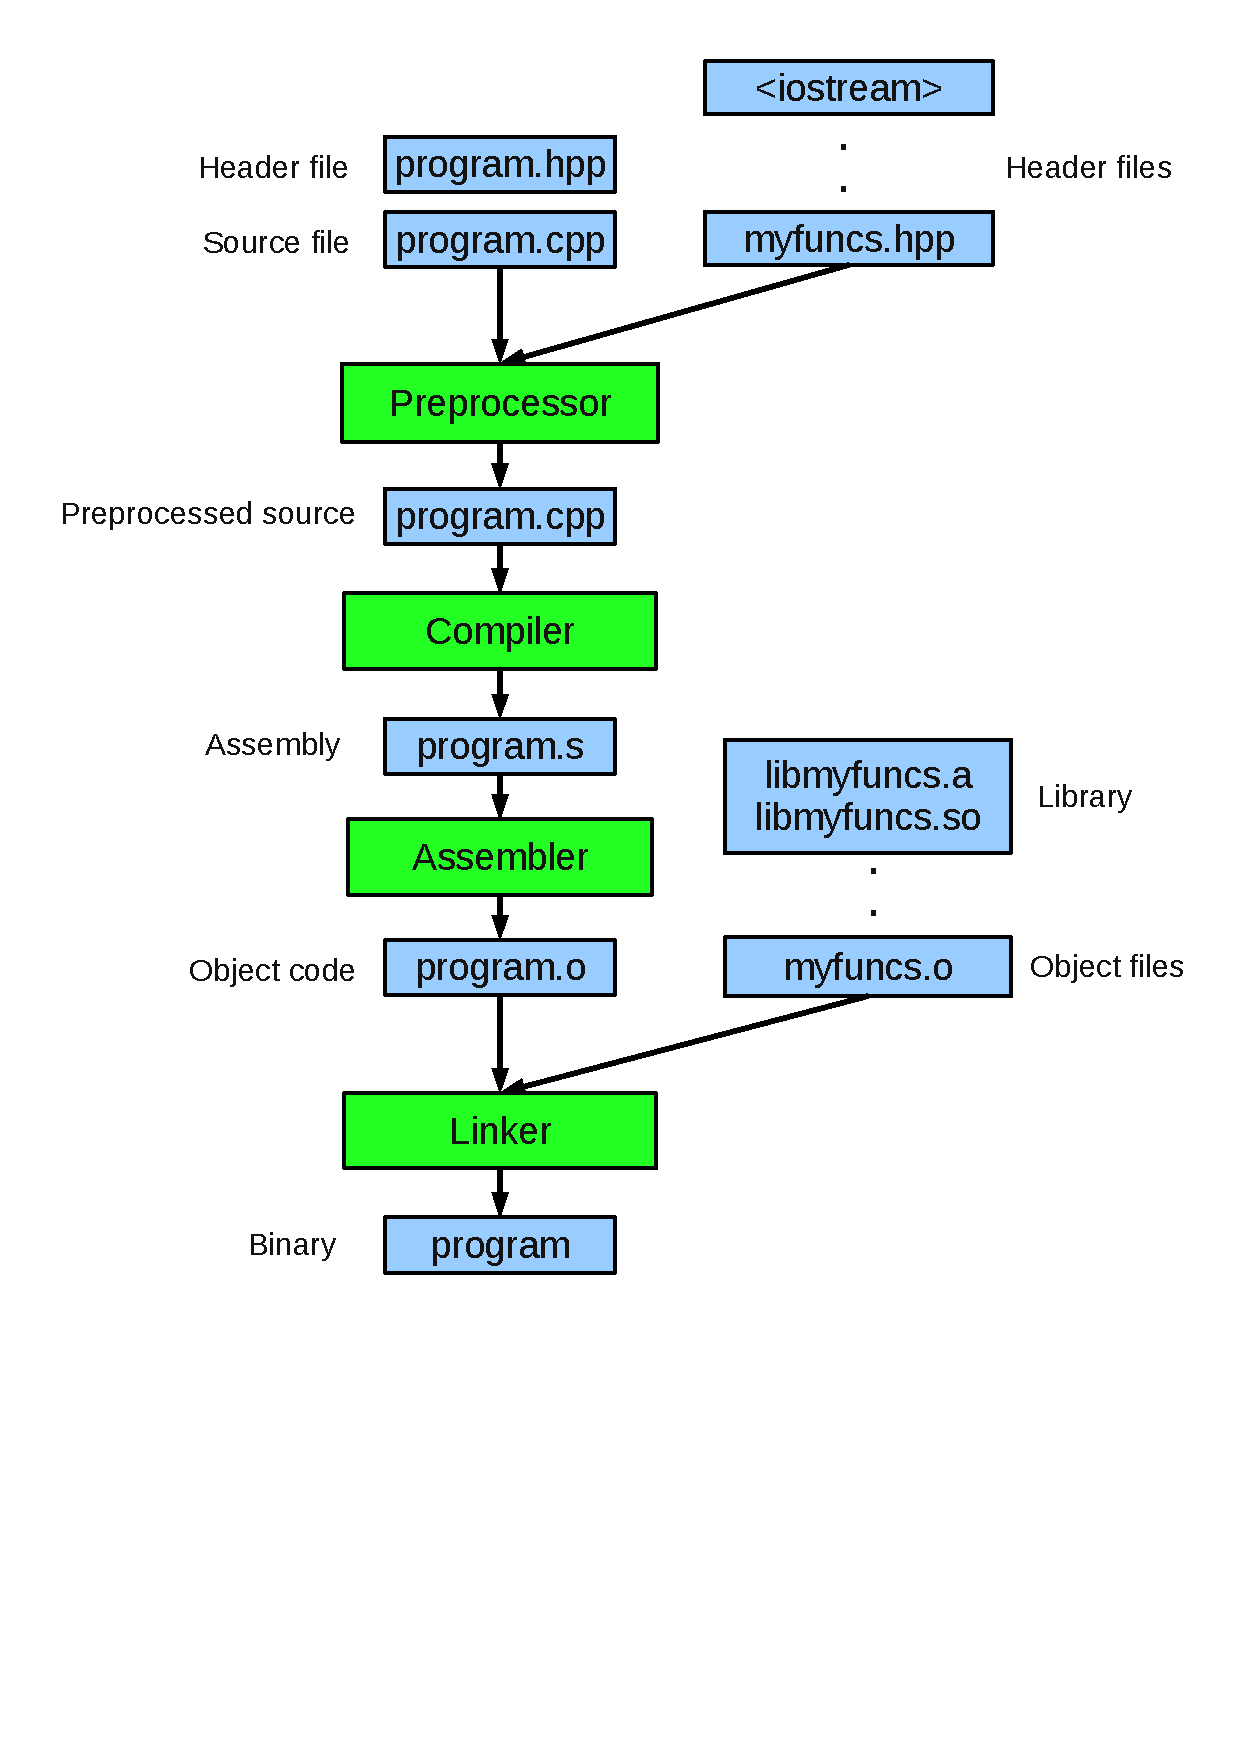
\includegraphics[height=1.1\textheight]{compilation}
  \end{columns}
\end{frame}

\begin{frame}[fragile]
  \frametitle{Libraries}
  \begin{columns}[T,onlytextwidth]
    \column{0.5\textwidth}
  \begin{itemize}
  \item \lstinline!ar! can put several object files together into a
    \emph{library}
  \item The name is \lstinline!lib<name>.a! or
    \lstinline!lib<name>.so! (\eg \lstinline!libgsl.a!)
  \item A library file should come together with a set of header files
    (\eg gsl.h)
  \item A library file can be linked together with other object files
    via the compiler option \texttt{-l<name>} (\eg \texttt{-lgsl})
  \end{itemize}
    \column{0.5\textwidth}
    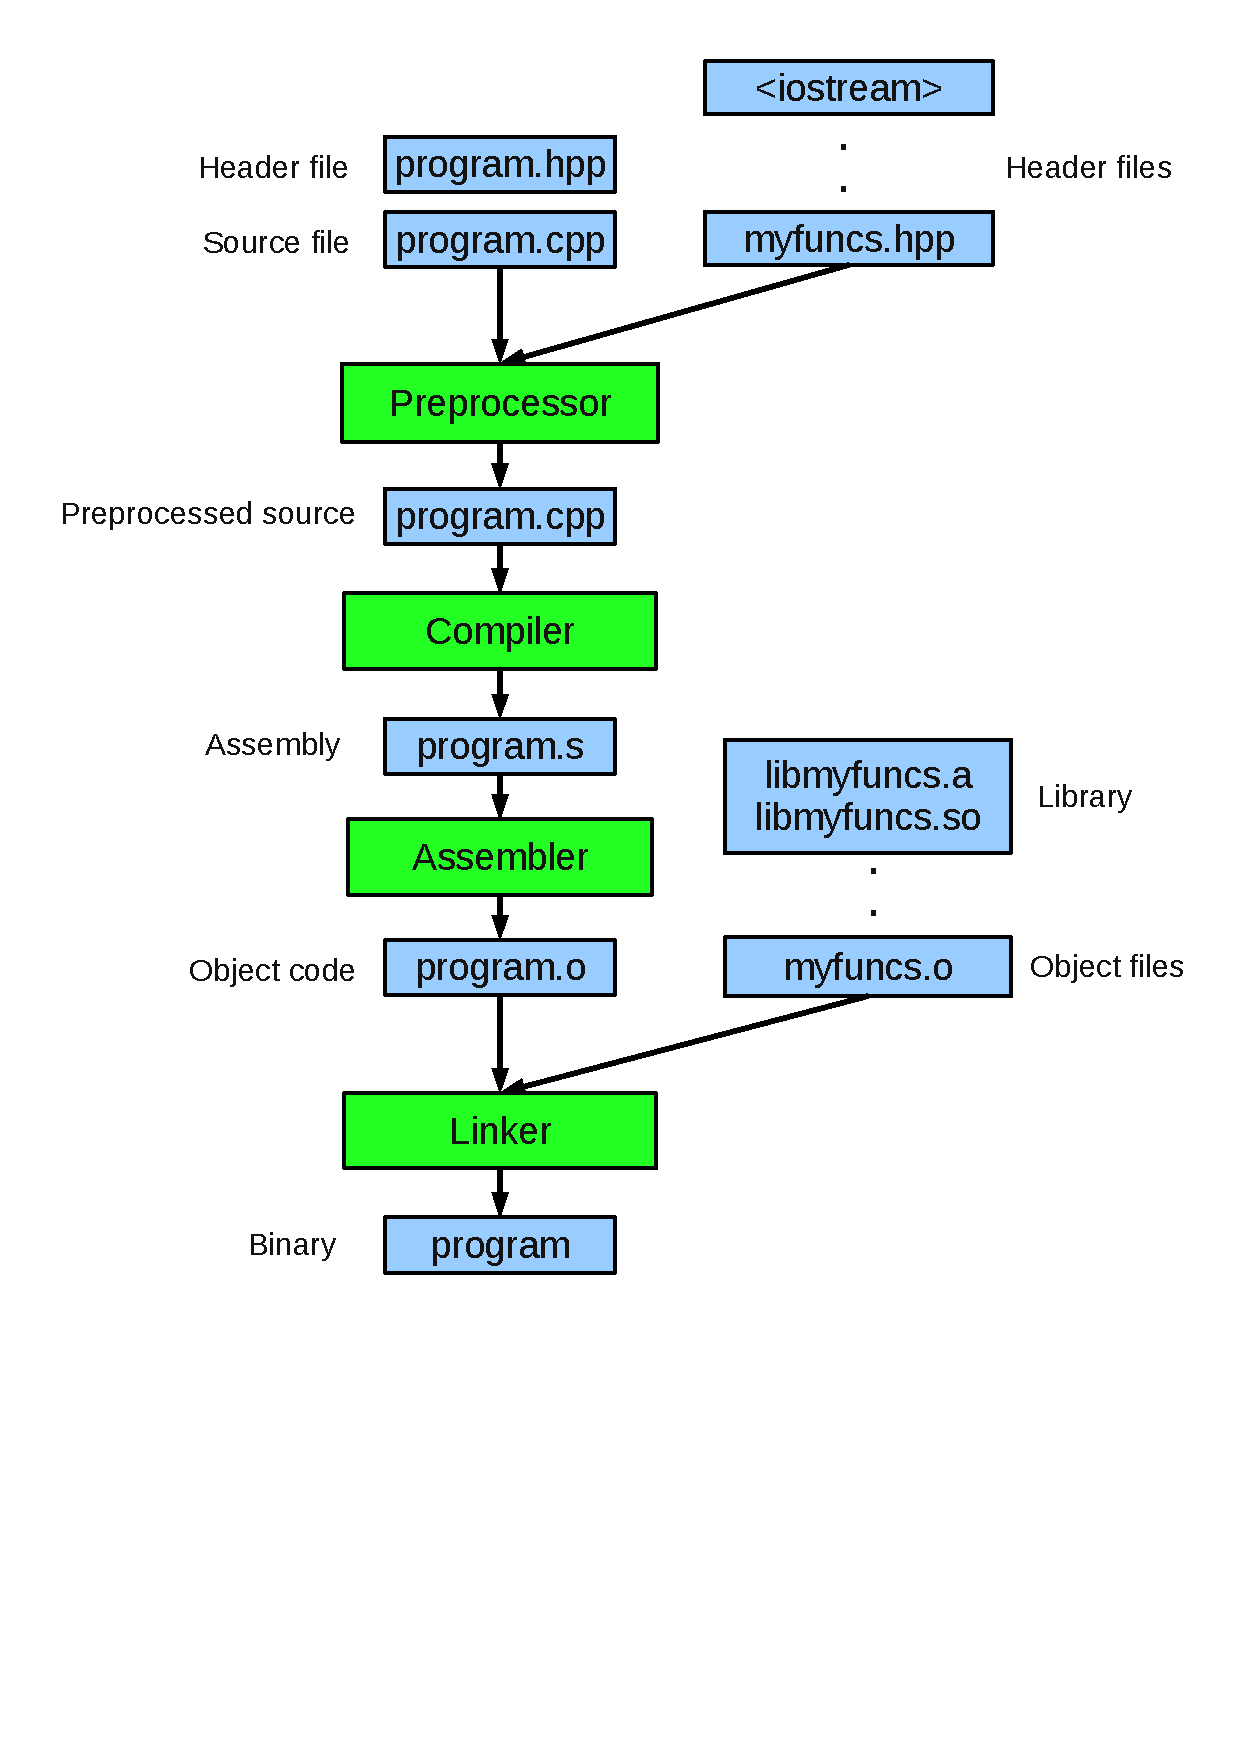
\includegraphics[height=1.1\textheight]{compilation}
  \end{columns}
\end{frame}


\end{document}
